% Options for packages loaded elsewhere
\PassOptionsToPackage{unicode}{hyperref}
\PassOptionsToPackage{hyphens}{url}
\documentclass[
  11pt,
]{article}
\usepackage{xcolor}
\usepackage[margin=22mm]{geometry}
\usepackage{amsmath,amssymb}
\setcounter{secnumdepth}{-\maxdimen} % remove section numbering
\usepackage{iftex}
\ifPDFTeX
  \usepackage[T1]{fontenc}
  \usepackage[utf8]{inputenc}
  \usepackage{textcomp} % provide euro and other symbols
\else % if luatex or xetex
  \usepackage{unicode-math} % this also loads fontspec
  \defaultfontfeatures{Scale=MatchLowercase}
  \defaultfontfeatures[\rmfamily]{Ligatures=TeX,Scale=1}
\fi
\usepackage{lmodern}
\ifPDFTeX\else
  % xetex/luatex font selection
\fi
% Use upquote if available, for straight quotes in verbatim environments
\IfFileExists{upquote.sty}{\usepackage{upquote}}{}
\IfFileExists{microtype.sty}{% use microtype if available
  \usepackage[]{microtype}
  \UseMicrotypeSet[protrusion]{basicmath} % disable protrusion for tt fonts
}{}
\makeatletter
\@ifundefined{KOMAClassName}{% if non-KOMA class
  \IfFileExists{parskip.sty}{%
    \usepackage{parskip}
  }{% else
    \setlength{\parindent}{0pt}
    \setlength{\parskip}{6pt plus 2pt minus 1pt}}
}{% if KOMA class
  \KOMAoptions{parskip=half}}
\makeatother
\usepackage{graphicx}
\makeatletter
\newsavebox\pandoc@box
\newcommand*\pandocbounded[1]{% scales image to fit in text height/width
  \sbox\pandoc@box{#1}%
  \Gscale@div\@tempa{\textheight}{\dimexpr\ht\pandoc@box+\dp\pandoc@box\relax}%
  \Gscale@div\@tempb{\linewidth}{\wd\pandoc@box}%
  \ifdim\@tempb\p@<\@tempa\p@\let\@tempa\@tempb\fi% select the smaller of both
  \ifdim\@tempa\p@<\p@\scalebox{\@tempa}{\usebox\pandoc@box}%
  \else\usebox{\pandoc@box}%
  \fi%
}
% Set default figure placement to htbp
\def\fps@figure{htbp}
\makeatother
\setlength{\emergencystretch}{3em} % prevent overfull lines
\providecommand{\tightlist}{%
  \setlength{\itemsep}{0pt}\setlength{\parskip}{0pt}}
\usepackage{bookmark}
\IfFileExists{xurl.sty}{\usepackage{xurl}}{} % add URL line breaks if available
\urlstyle{same}
\hypersetup{
  hidelinks,
  pdfcreator={LaTeX via pandoc}}

\author{}
\date{}

\begin{document}

\section{Weyl kernels, operator traces, and a finite trace-class
test}\label{weyl-kernels-operator-traces-and-a-finite-trace-class-test}

\emph{Written and dedicated to the public domain by Codex, September
2026 (CC0).}

A Weyl symbol lives on phase space, while its operator acts on a Hilbert
space. To compare their traces, we first identify every Hilbert--Schmidt
kernel and its exact Fourier factor. A trace-class operator with an
integrable Weyl symbol then has a phase-space trace, even when its
kernel has no continuous diagonal. Finally, a finite list of weighted
symbol derivatives gives a concrete trace-class test. The integer
\(n+1\) is forced by the oscillator spectrum in \(n\) configuration
variables; no index formula is needed for these results.

The needed course lessons are
\href{euclidean-symbol-calculus.pdf}{Symbols, operators and Sobolev
scales} for the Fourier convention \(D=-i\partial\), Weyl quantization,
Plancherel and symbolic composition, and
\href{traces-and-complexes.pdf}{Traces that survive passage to
cohomology} for Hilbert--Schmidt operators, trace-class products, polar
factorization and matrix traces. We prove the additional kernel,
diagonal and weighted-derivative steps here. This lesson concerns the
original matrix symbol on \(\mathbb R^{2n}_{x,\xi}\); the analytic index
integral requires further arguments.

\subsection{1. Hilbert--Schmidt maps and their complete
kernels}\label{hilbertschmidt-maps-and-their-complete-kernels}

Put \(H_\nu=L^2(\mathbb R^n;\mathbb C^\nu)\) and
\(H_\mu=L^2(\mathbb R^n;\mathbb C^\mu)\), with inner products linear in
the first variable. A measurable matrix kernel
\(K(x,y)\in\operatorname{Hom}(\mathbb C^\nu,\mathbb C^\mu)\) is squared
with its full Hilbert--Schmidt fiber norm
\(\operatorname{tr}_{\mathbb C^\nu}(K(x,y)^*K(x,y))\). If
\(K\in L^2(\mathbb R^{2n})\), Cauchy--Schwarz in \(y\) gives \[
 \|T_Ku\|_{H_\mu}^2
 \leq \|K\|_{L^2_{x,y};\mathrm{HS}}^2\,\|u\|_{H_\nu}^2,\qquad
 T_Ku(x)=\int_{\mathbb R^n}K(x,y)u(y)\,dy .
 \tag{CI1}
\] The integral exists for almost every \(x\). To recover the exact
Hilbert--Schmidt norm, take an orthonormal basis \((e_j)\) of \(H_\nu\).
For almost every \(x\), Parseval in the input Hilbert space identifies
\(\sum_j\|T_Ke_j(x)\|_{\mathbb C^\mu}^2\) with the squared \(L^2_y\)
norm of the whole matrix row \(K(x,\cdot)\). Tonelli then gives \[
 \|T_K\|_{\mathcal S_2(H_\nu,H_\mu)}^2
   =\sum_j\|T_Ke_j\|_{H_\mu}^2
   =\iint_{\mathbb R^{2n}}
       \operatorname{tr}_{\mathbb C^\nu}(K^*K)(x,y)\,dx\,dy.
 \tag{CI2}
\] Conversely, for an arbitrary Hilbert--Schmidt \(T:H_\nu\to H_\mu\),
the finite-rank kernel sums \[
 K_N(x,y)=\sum_{j=1}^N(Te_j)(x)e_j(y)^*
 \tag{CI3}
\] are Cauchy in the full matrix-valued \(L^2_{x,y}\) norm, since
orthonormality in \(y\) makes the squared norm of a tail equal to
\(\sum_{j=M+1}^N\|Te_j\|^2\). Let \(K\) be their \(L^2\) limit. Each
\(T_{K_N}\) agrees with \(T\) on the first \(N\) basis vectors, and
(CI1) makes \(T_{K_N}\to T_K\) in operator norm. Density of the finite
basis spans and the Hilbert--Schmidt bound make \(T=T_K\). Thus
square-integrable kernels and Hilbert--Schmidt maps are isometrically
the same objects, with no unmentioned smoothness assumption.

\subsection{2. The exact Weyl factor}\label{the-exact-weyl-factor}

Use the original Fourier convention \(D=-i\partial\) and inverse
coefficient \((2\pi)^{-n}\). For a matrix Weyl symbol \(a(u,\xi)\), its
kernel is the partial inverse Fourier transform \[
 K_{a^w}(x,y)
  =(2\pi)^{-n}\int_{\mathbb R^n}
      e^{i(x-y)\cdot\xi}\,
      a\!\left(\frac{x+y}{2},\xi\right)d\xi .
 \tag{CI4}
\] This first holds for Schwartz symbols. The linear change
\(u=(x+y)/2,\ v=x-y\) has absolute Jacobian one: in one coordinate pair
its inverse matrix
\(\left(\begin{smallmatrix}1&1/2\\1&-1/2\end{smallmatrix}\right)\) has
determinant \(-1\), and the \(n\) coordinate pairs multiply the absolute
values. Plancherel in \(v\), with the exact inverse Fourier coefficient
in (CI4), gives \[
 \|a^w\|_{\mathcal S_2(H_\nu)}^2
  =(2\pi)^{-n}\iint_{\mathbb R^{2n}}
       \operatorname{tr}_{\mathbb C^\nu}(a(u,\xi)^*a(u,\xi))
       \,du\,d\xi .
 \tag{CI5}
\] Schwartz functions are dense in matrix \(L^2(\mathbb R^{2n})\), and
both sides of (CI5) are complete. The partial Fourier transform in (CI4)
therefore extends the identity to every \(L^2\) Weyl symbol. Conversely
(CI3), followed by the invertible coordinate change and partial Fourier
transform, gives a unique \(L^2\) Weyl symbol for every Hilbert--Schmidt
operator. This also proves that the symbol-to-kernel map is injective at
the \(L^2\) level.

\subsection{3. Continuous trace-class kernels and their
diagonal}\label{continuous-trace-class-kernels-and-their-diagonal}

Let \(T:H_\nu\to H_\nu\) be trace class. Its polar factorization gives
\(T=AB\) with \(A=U|T|^{1/2}\) and \(B=|T|^{1/2}\), both
Hilbert--Schmidt; the trace lesson proves the exact norm identity and
finite-rank approximation used here. Let their \(L^2\) kernels be
\(A(x,z)\) and \(B(z,y)\). Cauchy--Schwarz in \(z\) makes \[
 K_T(x,y)=\int_{\mathbb R^n}A(x,z)B(z,y)\,dz
 \quad\text{for almost every }(x,y),
 \tag{CI6}
\] and bounds its absolute matrix norm by
\(\|A(x,\cdot)\|_{L^2_z}\|B(\cdot,y)\|_{L^2_z}\), an \(L^2_{x,y}\)
product. Fubini first proves that its operator is \(AB\) on compact
smooth tests; the \(L^2\) bound and density then prove it on all
\(H_\nu\). In particular this is the unique Hilbert--Schmidt kernel of
\(T\).

The diagonal factorization \(k(x)=\int A(x,z)B(z,x)\,dz\) is defined for
almost every \(x\). Matrix Cauchy--Schwarz and then scalar
Cauchy--Schwarz in \(x\) show \(k\in L^1_x\). Finite-rank kernel
approximation of \(A,B\), together with \(\|A_1B_1-A_2B_2\|_1
\leq\|A_1-A_2\|_2\|B_1\|_2+\|A_2\|_2\|B_1-B_2\|_2\), gives the exact
trace identity \[
 \operatorname{Tr}T
  =\int_{\mathbb R^n}\operatorname{tr}_{\mathbb C^\nu}
           \left(\int_{\mathbb R^n}A(x,z)B(z,x)\,dz\right)dx.
 \tag{CI7}
\] For finite rank this is a direct sum of rank-one inner products; the
displayed trace-norm bound and \(L^1\) bound pass the identity to the
Hilbert--Schmidt factors.

If the operator kernel has a continuous representative \(K_T(x,y)\), its
actual diagonal equals \(k(x)\) almost everywhere. Here is the step that
avoids assigning arbitrary values to an \(L^2\) kernel on a measure-zero
diagonal. Regard \(y\mapsto B(\cdot,y)\) as an \(L^2_z\)-valued
\(L^2_y\) function. At almost every \(x\), it has an \(L^2_z\)-valued
Lebesgue point \(y=x\), while \(A(x,\cdot)\in L^2_z\), and (CI6) holds
for almost every \(y\). Average (CI6) over a ball \(B_\varepsilon(x)\)
in \(y\). The average of \(B(\cdot,y)\) tends to \(B(\cdot,x)\) in
\(L^2_z\), so its pairing with \(A(x,\cdot)\) tends to \(k(x)\). The
continuous representative's average tends to \(K_T(x,x)\). Therefore \[
 \operatorname{Tr}T
   =\int_{\mathbb R^n}\operatorname{tr}_{\mathbb C^\nu}K_T(x,x)\,dx
 \quad\text{when }K_T\text{ has a continuous representative.}
 \tag{CI8}
\] The integral is absolutely defined because the diagonal agrees almost
everywhere with the \(L^1\) factorization in (CI7). No compactness of
\(\mathbb R^n\) or positivity of \(T\) was used.

\subsection{4. The trace of an integrable Weyl
symbol}\label{the-trace-of-an-integrable-weyl-symbol}

The diagonal argument in Section 3 does not automatically apply to a
trace-class Weyl operator with merely \(a\in L^1\); the kernel need not
be continuous. Use a coherent-state resolution that keeps the Weyl
coefficient. Let \(g(x)=\pi^{-n/4}e^{-|x|^2/2}\), \(\|g\|_2=1\), and
\(g_{q,p}(x)=e^{ip\cdot(x-q/2)}g(x-q)\). Fourier inversion in \(p\),
followed by \(\int|g(x-q)|^2dq=1\), proves for \(u,v\in\mathcal S\) and
then for all \(L^2\) vectors that \[
 (2\pi)^{-n}\iint_{\mathbb R^{2n}}
       \langle u,g_{q,p}\rangle
       \langle g_{q,p},v\rangle\,dq\,dp
   =\langle u,v\rangle .
 \tag{CI9}
\] The phases involving \(q/2\) cancel in this product. Cauchy--Schwarz
and (CI9) give an absolute integral bound
\((2\pi)^{-n}\int|\langle w,g_{q,p}\rangle
\langle g_{q,p},v\rangle|\,dq\,dp\leq\|w\|_2\|v\|_2\). Expand a
trace-class \(T\) as a trace-norm convergent sum of rank-one maps with
total coefficient sum \(\|T\|_1\). The bound permits termwise
integration and proves \[
 \operatorname{Tr}T
   =(2\pi)^{-n}\iint
          \langle Tg_{q,p},g_{q,p}\rangle\,dq\,dp .
 \tag{CI10}
\] For \(H_\nu\), sum this identity over the standard fiber basis
\(e_\alpha\), \(1\leq\alpha\leq\nu\); every fiber index remains present.

For a Schwartz Weyl symbol, insert (CI4) into the quadratic pairing and
set \(u=(x+y)/2,\ v=x-y\). The Wigner factor of \(g_{q,p}\) is computed
by one complete Gaussian Fourier integral: \[
 W_{g_{q,p}}(u,\xi)
 =\int e^{-iv\cdot\xi}
       g_{q,p}(u+v/2)\overline{g_{q,p}(u-v/2)}\,dv
 =2^n e^{-|u-q|^2-|\xi-p|^2}.
 \tag{CI11}
\] Hence \(\langle a^wg_{q,p},g_{q,p}\rangle
=(2\pi)^{-n}\int a(u,\xi)W_{g_{q,p}}(u,\xi)\,du\,d\xi\). The same
identity holds for any integrable matrix symbol \(a\): the Gaussian
Wigner factor is bounded, the kernel identity is distributional, and
approximation of \(a\) in \(L^1\) makes the pairing converge. Integrate
\(q,p\) in (CI11): \(\int 2^n e^{-|u-q|^2-|\xi-p|^2}\,dq\,dp
=2^n\pi^n=(2\pi)^n\), independently of \(u,\xi\). Absolute Fubini
follows from \(a\in L^1\). If \(a^w\) is also trace class, (CI10)
therefore gives the exact formula \[
 \operatorname{Tr}a^w
   =(2\pi)^{-n}\iint_{\mathbb R^{2n}}
          \operatorname{tr}_{\mathbb C^\nu}a(u,\xi)\,du\,d\xi .
 \tag{CI12}
\] The hypotheses ``\(a\in L^1\)'' and ``\(a^w\) trace class'' play
different roles and are both retained. Formula (CI12) has not inferred
trace class from \(L^1\) alone.

The constants can be checked without a limiting argument on the full
Gaussian \(a(u,\xi)=e^{-|u|^2-|\xi|^2}\). Its \(\xi\) integral in (CI4)
gives \(K_{a^w}(x,y)=2^{-n}\pi^{-n/2}e^{-(|x|^2+|y|^2)/2}
=2^{-n}g(x)\overline{g(y)}\), because
\(|(x+y)/2|^2+|x-y|^2/4=(|x|^2+|y|^2)/2\). Thus it is the rank-one
orthogonal projection onto \(g\), multiplied by \(2^{-n}\). The two
independently proved formulas give exactly \[
 \operatorname{Tr}a^w=2^{-n}
   =(2\pi)^{-n}\iint e^{-|u|^2-|\xi|^2}\,du\,d\xi,
 \qquad
 \|a^w\|_2^2=4^{-n}
   =(2\pi)^{-n}\iint e^{-2|u|^2-2|\xi|^2}\,du\,d\xi.
 \tag{CI13}
\]

\subsection{5. The full finite seminorm and the
claim}\label{the-full-finite-seminorm-and-the-claim}

Let \(n,\nu\ge1\), \(z=(x,\xi)\in\mathbb R^{2n}\), and let
\(a(z)\in\operatorname{End}(\mathbb C^\nu)\) be a smooth matrix symbol
for which the following full finite sum is finite: \[
 \mathcal N_{n+1}(a)
 =\sum_{\substack{\alpha,\beta,\alpha',\beta'\in\mathbb N^n\\
      |\alpha|+|\beta|+|\alpha'|+|\beta'|\le n+1}}
   \left\|x^\alpha\xi^\beta
      \partial_x^{\alpha'}\partial_\xi^{\beta'}a(x,\xi)
   \right\|_{L^2(\mathbb R^{2n};\mathrm{HS}_{\nu})}.
 \tag{CT1}
\] The operator \(a^w\) is then trace class on
\(L^2(\mathbb R^n;\mathbb C^\nu)\), and \[
 \|a^w\|_{\mathcal S_1}
    \le C_{n,\nu}\mathcal N_{n+1}(a).
 \tag{CT2}
\] The proof uses the exact positive oscillator, not a replacement of
the original symbol by a completed or rescaled object. We will also
prove that (CT1) makes \(a\in L^1\), so the actual trace is the original
phase-space integral from CI12.

\subsection{6. Oscillator eigenvectors and the Hilbert--Schmidt
inverse}\label{oscillator-eigenvectors-and-the-hilbertschmidt-inverse}

On \(\mathcal S(\mathbb R^n)\) put \[
 H=I+\sum_{j=1}^n(x_j^2+D_j^2)
   =I+|x|^2-\Delta_x,\qquad
 c_j=\frac{x_j+\partial_{x_j}}{\sqrt2},\qquad
 c_j^*=\frac{x_j-\partial_{x_j}}{\sqrt2}.
 \tag{CT3}
\] Integration by parts makes \(c_j^*\) the Hilbert adjoint of \(c_j\)
on Schwartz vectors. The derivative identity
\(\partial_{x_j}x_j=x_j\partial_{x_j}+I\) gives
\([c_i,c_j^*]=\delta_{ij}I\), all other creation/annihilation
commutators zero, and the exact unshifted identity \[
 H=(n+1)I+2\sum_{j=1}^n c_j^*c_j.
 \tag{CT4}
\] Let \(g(x)=\pi^{-n/4}e^{-|x|^2/2}\). It has norm one and \(c_jg=0\).
Repeatedly commute each annihilator through the creators and use
\(c_jg=0\) to see that \[
 h_\gamma=(\gamma!)^{-1/2}
       (c_1^*)^{\gamma_1}\cdots(c_n^*)^{\gamma_n}g,
 \qquad
 \langle h_\gamma,h_\delta\rangle=\delta_{\gamma\delta},
 \qquad
 Hh_\gamma=(n+1+2|\gamma|)h_\gamma.
 \tag{CT5}
\] These vectors are complete. The creators generate Gaussian times
polynomials with triangular nonzero leading terms, hence their span is
exactly the span of \(x^\alpha g(x)\). If \(f\in L^2\) is orthogonal to
every \(x^\alpha g\), set \(F(w)=\int f(x)g(x)e^{w\cdot x}dx\) for
\(w\in\mathbb C^n\). Cauchy--Schwarz against the Gaussian gives absolute
convergence locally uniformly in \(w\), and the same bound after
arbitrary \(w\)-derivatives. Every Taylor coefficient at zero vanishes
by orthogonality, so successive one-variable entire-function uniqueness
gives \(F=0\). On \(w=it\), this is the Fourier transform of the \(L^1\)
function \(fg\), hence Fourier injectivity gives \(fg=0\) almost
everywhere and \(f=0\). Thus (CT5) is an orthonormal basis. Its diagonal
operator is selfadjoint on the coefficient domain
\(\sum_\gamma(n+1+2|\gamma|)^2|u_\gamma|^2<\infty\); finite Hermite sums
are a graph core by truncation. For any Schwartz \(u\), integration by
parts against \(h_\gamma\) shows the coefficients of the differential
expression \(Hu\) are \((n+1+2|\gamma|)u_\gamma\), so
\(H|_{\mathcal S}\) lies inside that diagonal operator. Since the finite
Hermite core lies inside \(\mathcal S\), its closure is exactly the
diagonal selfadjoint operator. This proves the real spectral powers used
below.

Take the integer \(k=n+1\). On the full vector-valued Hilbert space,
(CT5) gives \[
 \|H^{-k/2}\otimes I_\nu\|_{\mathcal S_2}^2
 =\nu\sum_{\gamma\in\mathbb N^n}(n+1+2|\gamma|)^{-k}
 <\infty.
 \tag{CT6}
\] Indeed the number of \(\gamma\) with \(|\gamma|=r\) is
\(\binom{r+n-1}{n-1}\le C_n(1+r)^{n-1}\). The shell sum is bounded by
\(C\sum_{r\ge0}(1+r)^{n-1-k}=C\sum_{r\ge0}(1+r)^{-2}\), including
\(n=1\). This is the exact reason the threshold is \(k=n+1\).

\subsection{7. The integer oscillator graph
estimate}\label{the-integer-oscillator-graph-estimate}

For each \(j\), the ladder relation from (CT5) is \[
 (c_j^*)^k h_\gamma
 =\left(\frac{(\gamma_j+k)!}{\gamma_j!}\right)^{1/2}
          h_{\gamma+ke_j}.
 \tag{CT7}
\] Fix \(\gamma\) and choose \(j\) with \(\gamma_j\ge|\gamma|/n\). Then
\((\gamma_j+k)!/\gamma_j!\ge(\gamma_j+1)^k
\ge c_{n,k}(1+|\gamma|)^k\). The other direction follows from each
factor \(\gamma_j+\ell\le|\gamma|+k\). Since \(H\) has eigenvalue
\(n+1+2|\gamma|\), the coefficient comparison, summed against the
squared Hermite coefficients of \(u\), proves \[
 \|H^{k/2}u\|_2^2
 \le C_{n,k}\sum_{j=1}^n\|(c_j^*)^k u\|_2^2
 \quad (u\in\mathcal S).
 \tag{CT8}
\] This is an integer-order estimate although \(H^{k/2}\) need not be a
differential operator when \(k\) is odd. No fractional-symbol formula
has been assumed.

By (CT3), each \((c_j^*)^k=2^{-k/2}(x_j-\partial_{x_j})^k\).
Noncommutative expansion by induction, moving each derivative past each
multiplication using \(\partial_{x_j}x_j=x_j\partial_{x_j}+I\), writes
it as a finite linear combination of \(x_j^r\partial_{x_j}^s\) with
\(r+s\le k\), including all lower commutator terms. Applying the
triangle inequality to (CT8) gives the exact graph estimate \[
 \|H^{k/2}u\|_2
 \le C_{n,k}\sum_{\substack{\alpha,\beta\in\mathbb N^n\\
                         |\alpha|+|\beta|\le k}}
          \|x^\alpha D^\beta u\|_2 .
 \tag{CT9}
\] All coefficients and commutator terms are finite constants depending
only on \(n,k\).

\subsection{8. Original Weyl symbol under each output
weight}\label{original-weyl-symbol-under-each-output-weight}

For a Schwartz matrix symbol \(a\), start from its actual kernel (CI4),
write \(z=(x+y)/2\) and \(v=x-y\), and differentiate or integrate by
parts in the phase \(e^{iv\cdot\xi}\). Multiplication by the output
\(x_j=z_j+v_j/2\) and
\(v_je^{iv\cdot\xi}=-i\partial_{\xi_j}e^{iv\cdot\xi}\) gives the exact
left-action identity \[
 x_j a^w
   =\left(z_j a+\frac{i}{2}\partial_{\xi_j}a\right)^w,
 \qquad
 D_j a^w
   =\left(\xi_j a-\frac{i}{2}\partial_{z_j}a\right)^w .
 \tag{CT10}
\] The second follows by differentiating both \(e^{iv\cdot\xi}\) and
\(a(z,\xi)\) with respect to the output \(x_j\), retaining the factor
\(1/2\) in \(\partial_{x_j}z_j\). These formulas hold entrywise for
matrices; no matrix factors are commuted. Repeated action in the
displayed operator order shows that the Weyl symbol of every
\(x^\alpha D^\beta a^w\), \(|\alpha|+|\beta|\le k\), is a finite sum of
terms \[
 C\,z^\rho\xi^\sigma
       \partial_z^{\rho'}\partial_\xi^{\sigma'}a,
 \qquad
 |\rho|+|\sigma|+|\rho'|+|\sigma'|
       \le|\alpha|+|\beta|\le k.
 \tag{CT11}
\] The bound is proved by induction on the word length: each application
in (CT10) adds one multiplication or one derivative; when the derivative
hits an earlier polynomial weight, both counts decrease by one. Thus no
hidden term can exceed the total degree \(k\) in (CT1).

The graph estimate applies to every output used in this step. For
Schwartz \(a\), formula (CI4), its partial Fourier transform and its
invertible linear coordinate change give
\(K_{a^w}\in\mathcal S(\mathbb R^{2n})\). For every \(f\in L^2\), every
output derivative and every polynomial output weight, differentiating
the kernel integral gives \[
 \sup_x\left|x^\alpha\partial_x^\beta(a^wf)(x)\right|
 \leq\sup_x\left\|x^\alpha\partial_x^\beta K_{a^w}(x,\cdot)
          \right\|_{L^2_y;\mathrm{HS}}\|f\|_2<\infty.
 \tag{CT11a}
\] The right side is finite because the full kernel is Schwartz; a fixed
sufficiently high power of \(1+|y|\) bounds its squared row integral
uniformly in \(x\). The same domination justifies differentiation under
that integral at every order. Thus \(a^wf\) is a Schwartz vector, even
when \(f\) is an arbitrary orthonormal basis vector. This establishes
the actual graph domain before applying (CT9).

Apply the proven Weyl Hilbert--Schmidt identity CI5 separately to every
term in (CT11), then use (CT9) on each output \(a^w e_\ell\) of an
orthonormal input basis. Tonelli permits the sum of nonnegative squared
norms, and finite-dimensional Cauchy--Schwarz absorbs the finite number
of terms: \[
 \|H^{k/2}a^w\|_{\mathcal S_2}
 \le C_{n,\nu}\mathcal N_k(a).
 \tag{CT12}
\] The full original \((2\pi)^{-n/2}\) factor from CI5 is inside
\(C_{n,\nu}\); it was not set equal to one in the proof.

\subsection{9. Factorization, density, and the actual
trace}\label{factorization-density-and-the-actual-trace}

On Schwartz inputs, insert the exact spectral identity \[
 a^w=(H^{-k/2}\otimes I_\nu)
             (H^{k/2}\otimes I_\nu)a^w .
 \tag{CT13}
\] The first factor is Hilbert--Schmidt by (CT6); the second is
Hilbert--Schmidt by (CT12). The Hilbert-ideal product inequality from
the owned trace lesson therefore proves (CT2), with no claim that either
factor is bounded by its symbol's pointwise supremum.

For completeness, smooth compactly supported matrix symbols are dense in
the norm (CT1) among smooth symbols with finite (CT1). Multiply \(a\) by
a radial cutoff \(\chi(z/R)\) equal to one on \(|z|\le R\). An
undifferentiated weighted term converges by dominated convergence. If
\(j\ge1\) derivatives hit the cutoff, their factor is \(O(R^{-j})\) on
\(R\lesssim|z|\lesssim2R\); there \(R^{-j}\le C\langle z\rangle^{-j}\).
Multiplying this by an original weight monomial of degree \(d\) bounds
it by a finite sum of weight monomials of degree at most \(d\), times a
lower derivative of \(a\) whose total weighted/derivative degree remains
at most \(k\). Its \(L^2\) tail tends to zero. After cutoff, ordinary
smooth mollification converges in every derivative \(L^2\) norm through
order \(k\), and all polynomial weights are bounded on one fixed
enlarged support. The resulting compact smooth approximants \(a_R\)
satisfy \(\mathcal N_k(a_R-a)\to0\). Equations (CI5) and (CT2) extend
the trace-class operator and the bound to the original symbol.

Finally (CT1) itself supplies the integrability needed for the trace
formula. In \(2n\) phase dimensions, \(k=n+1>n\), so
\(\int_{\mathbb R^{2n}}\langle z\rangle^{-2k}dz<\infty\). The polynomial
inequality \(\langle z\rangle^{2k}\le C_k\sum_{|\rho|+|\sigma|\le k}
|x^\rho\xi^\sigma|^2\) follows by expanding \((1+|x|^2+|\xi|^2)^k\) with
the multinomial theorem. Cauchy--Schwarz therefore yields \[
 \|a\|_{L^1_{z};\mathrm{HS}_\nu}
 \le
 \left(\int\langle z\rangle^{-2k}dz\right)^{1/2}
 \|\langle z\rangle^k a\|_{L^2_z;\mathrm{HS}_\nu}
 \le C_{n,\nu}\mathcal N_k(a).
 \tag{CT14}
\] Apply CI12 to the now proved trace-class \(a^w\) and the actual
integrable symbol \(a\): \[
 \operatorname{Tr}a^w
  =(2\pi)^{-n}
       \iint_{\mathbb R^{2n}}
          \operatorname{tr}_{\mathbb C^\nu}a(x,\xi)\,dx\,d\xi .
 \tag{CT15}
\] The quantitative estimate (CT2) and trace identity (CT15) use the
original matrix-valued Weyl symbol and exactly the finite threshold in
(CT1).

\subsection{10. Worked example: a rationally decaying matrix
symbol}\label{worked-example-a-rationally-decaying-matrix-symbol}

For \(M>n+\tfrac12\), keep the full scalar function and matrix rank \[
 a_M(x,\xi)
   =\bigl(1+|x|^2+|\xi|^2\bigr)^{-M}I_\nu
   \quad\text{on }\mathbb R^{2n}.
 \tag{WT1}
\] Every differentiated factor can be obtained by repeated product and
chain rules, giving \[
 |\partial_{x,\xi}^{\gamma}a_M(z)|_{\mathrm{HS}_\nu}
   \le C_{M,\gamma,\nu}\langle z\rangle^{-2M-|\gamma|},
 \qquad \langle z\rangle=(1+|x|^2+|\xi|^2)^{1/2}.
 \tag{WT2}
\] To see the bound without hiding a term, a derivative of order \(j\)
is a finite sum of expressions
\(Cz^\delta(1+|z|^2)^{-M-(j+|\delta|)/2}\) with \(|\delta|\le j\) and
\(j+|\delta|\) even; each has the displayed decay. For a term in (CT1)
with polynomial weight degree \(d\) and derivative degree \(j\), where
\(d+j\le n+1\), (WT2) bounds its Hilbert--Schmidt norm by
\(C\langle z\rangle^{-2M+d-j}\). The largest exponent occurs at
\(d=n+1,j=0\). In \(2n\) dimensions its square is integrable exactly
when \(2(-2M+n+1)+2n<0\), or \(M>n+\tfrac12\). Thus the \textbf{full}
finite seminorm \(\mathcal N_{n+1}(a_M)\) is finite, and (CT2) proves
\(a_M^w\) is trace class.

The trace can now be computed from (CT15), without a diagonal regularity
assumption. Polar integration and \(t=r^2\) give \[
 \begin{aligned}
 \operatorname{Tr}a_M^w
  &=(2\pi)^{-n}\nu
      \int_{\mathbb R^{2n}}(1+|z|^2)^{-M}\,dz\\
  &=(2\pi)^{-n}\nu
      \frac{2\pi^n}{\Gamma(n)}
      \frac12\int_0^\infty t^{n-1}(1+t)^{-M}\,dt\\
  &=(2\pi)^{-n}\nu\pi^n
      \frac{\Gamma(M-n)}{\Gamma(M)} .
 \end{aligned}
 \tag{WT3}
\] The sphere-area factor follows by computing the Gaussian integral in
Cartesian and polar coordinates; the last integral is the beta integral
with the original exponents \(n-1\) and \(-M\). Its \(M>n\) convergence
condition is separately satisfied by the stronger trace-class criterion
used here.

\subsubsection{The exact trace-class threshold of the same rational
symbol}\label{the-exact-trace-class-threshold-of-the-same-rational-symbol}

The finite-derivative test above is sufficient. The actual original
symbol (WT1) has the stronger, exact classification \[
 a_M^w\text{ is trace class on }H_\nu
             \quad\Longleftrightarrow\quad M>n,
             \qquad M\in\mathbb R.                            \tag{WT6}
\] We retain \(a_M=(1+|x|^2+|\xi|^2)^{-M}I_\nu\), its matrix rank, Weyl
convention, and every phase-space factor. For \(n<M\leq n+1/2\), the
finite seminorm (CT1) is not finite, but the operator is still trace
class. This does not change the statement or proof of (CT2).

For \(t>0\), let \(T_t=(e^{-t(|x|^2+|\xi|^2)})^w\) on the scalar
configuration Hilbert space. The complete Gaussian Fourier integral in
(CI4) gives \[
 K_t(x,y)=(2\pi)^{-n}\left(\frac\pi t\right)^{n/2}
 \exp\left(-t\left|\frac{x+y}{2}\right|^2
                 -\frac{|x-y|^2}{4t}\right).                  \tag{WT7}
\] Put \(q_t=(1-t)/(1+t)\), retaining its sign. Use the actual Hermite
basis (CT5). Its generating vector is \[
 F_z(x)=g(x)\exp\left(\sqrt2\,z\cdot x-\frac{z\cdot z}{2}\right)
       =\sum_{\gamma\in\mathbb N^n}
          \frac{z^\gamma}{\sqrt{\gamma!}}h_\gamma(x),\qquad
 T_tF_z=(1+t)^{-n}F_{q_tz}.                                   \tag{WT8}
\] Here \(z\cdot z=\sum_jz_j^2\), without complex conjugation. The first
identity is proved by differentiating: \(\partial_{z_j}F_z=c_j^*F_z\)
and \(F_0=g\). Gaussian domination makes \(F_z\) an entire
\(L^2\)-valued function, so its Taylor coefficients are precisely the
creators in (CT5), with the displayed factorials.

To verify the second identity rather than importing a kernel summation
formula, insert \(F_z\) into (WT7). The coefficient of \(|y|^2\) in the
combined negative exponent is \((1+t)^2/(4t)\), and the linear term is
\(((t^{-1}-t)/2)x\cdot y+\sqrt2 z\cdot y\). Completing this Gaussian
square retains the integral factor \((4\pi t/(1+t)^2)^{n/2}\).
Multiplied by the coefficient in (WT7), it is \((1+t)^{-n}\). The
remaining exponent is exactly
\(-|x|^2/2+\sqrt2 q_tz\cdot x-q_t^2(z\cdot z)/2\), together with the
original normalization of \(g\). This proves (WT8). Differentiating it
at \(z=0\) gives the complete diagonal action \[
 \begin{gathered}
 T_th_\gamma=(1+t)^{-n}q_t^{|\gamma|}h_\gamma,\\
 \|T_t\otimes I_\nu\|_1
 =\nu(1+t)^{-n}\sum_{\gamma\in\mathbb N^n}|q_t|^{|\gamma|}
 =\nu(1+t)^{-n}(1-|q_t|)^{-n}\\
 =\begin{cases}
       \nu(2t)^{-n},&0<t\leq1,\\
       \nu\,2^{-n},&1\leq t<\infty.
   \end{cases}
 \end{gathered}                                                  \tag{WT9}
\] The sum is the product of \(n\) convergent geometric series, since
\(|q_t|<1\). At \(t=1\), \(q_t=0\), the zero-degree eigenvalue is
\(2^{-n}\), and every other eigenvalue is zero, exactly as in (CI13).
For \(t>1\), odd total degrees have negative eigenvalues; taking
absolute values in (WT9) is required. On a compact subinterval of
\(t>0\), the geometric tails are uniform and each eigenvalue is
continuous. Hence \(t\mapsto T_t\otimes I_\nu\) is continuous in trace
norm.

For \(M>n\), the original Gamma integral gives, pointwise and as a
tempered distribution, \[
 \begin{split}
 a_M(x,\xi)&=\frac1{\Gamma(M)}
    \int_0^\infty t^{M-1}e^{-t}
            e^{-t(|x|^2+|\xi|^2)}I_\nu\,dt,\\
 a_M^w&=\frac1{\Gamma(M)}
    \int_0^\infty t^{M-1}e^{-t}(T_t\otimes I_\nu)\,dt,\\
 \|a_M^w\|_1&\leq\frac{\nu}{2^n\Gamma(M)}
     \left(\int_0^1t^{M-n-1}e^{-t}\,dt
                     +\int_1^\infty t^{M-1}e^{-t}\,dt\right)<\infty.
 \end{split}                                                     \tag{WT10}
\] The second integral is a trace-norm integral, whose convergence
follows from every original factor in (WT9). It can be defined by
ordinary compact-interval Riemann sums in the complete trace ideal,
followed by the two norm-convergent endpoint limits. Its identification
with the original Weyl operator is exact: pair both sides with Schwartz
input and output vectors, use their Schwartz Wigner function and (CI4),
and apply absolute Fubini. The Gaussian symbol is bounded by one, while
\(t^{M-1}e^{-t}\) is integrable; the Wigner function has finite absolute
integral. The resulting pairing is that of the original Gamma integral.
Distributional kernel uniqueness therefore identifies this trace-class
map with \(a_M^w\), rather than with a different quantization. Since
\(M>n\) also gives \(a_M\in L^1\), its trace is the full original
expression (WT3) for every \(M>n\).

For necessity, let \(M\) be any real number and suppose this original
Weyl operator is trace class. The scalar symbol
\((1+|x|^2+|\xi|^2)^{-M}\) is positive and has at most polynomial
growth. Thus its pairing with the positive Gaussian Wigner function
(CI11) is absolutely defined at every coherent state, even when the
symbol is not integrable. Approximation against that Schwartz Wigner
function proves the same Weyl pairing identity directly. Sum over the
\(\nu\) fiber vectors in (CI10); every diagonal pairing is nonnegative.
Absolute integrability of those pairings would imply, by nonnegative
Tonelli and the complete Gaussian integral in (CI11), \[
 \begin{split}
 \|a_M^w\|_1
 &\geq(2\pi)^{-n}\int_{\mathbb R^{2n}}
     \sum_{\alpha=1}^{\nu}
     \left|\langle a_M^w(g_{q,p}e_\alpha),
                       g_{q,p}e_\alpha\rangle\right|\,dq\,dp\\
 &=(2\pi)^{-n}\nu\int_{\mathbb R^{2n}}
                     (1+|x|^2+|\xi|^2)^{-M}\,dx\,d\xi.
 \end{split}                                                     \tag{WT11}
\] The first inequality is the absolute rank-one integral bound proved
before (CI10), summed along a singular-value expansion. In \(2n\) phase
dimensions, the last radial integral converges exactly when \(2M>2n\);
at \(M=n\) its radial tail is logarithmically divergent, and for \(M<n\)
it diverges by a power. Consequently \(M\leq n\) contradicts finite
trace norm. This proves both directions of (WT6).

\begin{figure}
\centering
\pandocbounded{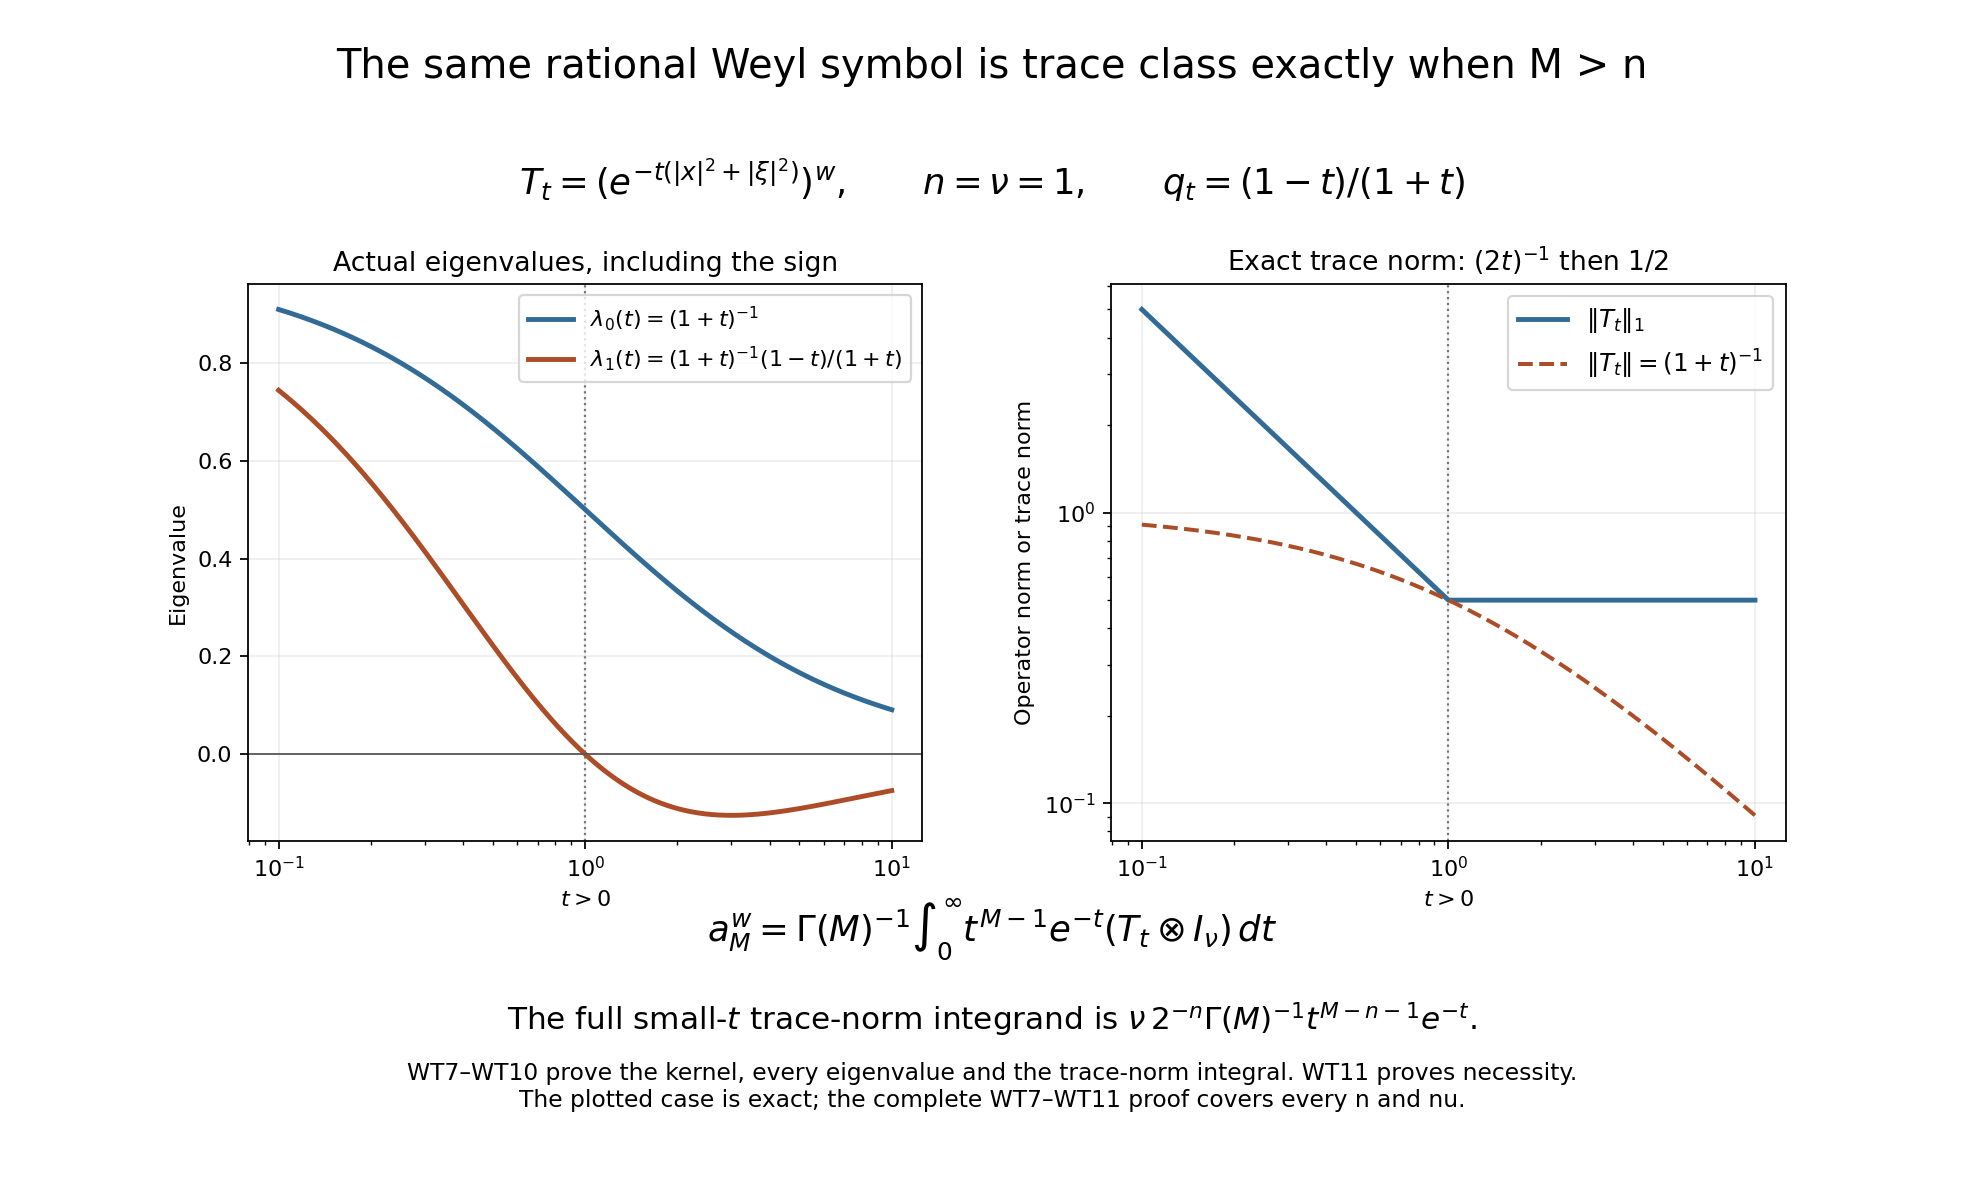
\includegraphics[keepaspectratio,alt={The exact Gaussian eigenvalues and trace norms used in the rational threshold proof}]{../figures/rational-weyl-trace.png}}
\caption{The exact Gaussian eigenvalues and trace norms used in the
rational threshold proof}
\end{figure}

The drawing uses the explicit case \(n=\nu=1\). It records the actual
sign change of the degree-one eigenvalue at \(t=1\) and the trace norm
from (WT9), including its factor \(1/2\). The rational-symbol
classification follows from the full endpoint integral (WT10) and the
positive coherent-state integral (WT11), not from a plotted sample. This
is an editorial strengthening of the worked example. The original
finite-derivative criterion remains identifiable; no novelty claim is
made.

\subsection{11. Exercises and complete
solutions}\label{exercises-and-complete-solutions}

\textbf{Exercise 1.} Let \(u\in L^2(\mathbb R^n;\mathbb C^\mu)\) and
\(v\in L^2(\mathbb R^n;\mathbb C^\nu)\). The rank-one map
\(S_{u,v}:H_\nu\to H_\mu\) is \(S_{u,v}w=u\langle w,v\rangle\), with the
lesson's inner product linear in its first variable. Find its kernel and
Hilbert--Schmidt norm. In the square case \(\mu=\nu\), find its trace.

\textbf{Solution.} The kernel is the full rectangular matrix
\(K(x,y)=u(x)v(y)^*\), so \[
 \iint\operatorname{tr}_{\mathbb C^\nu}(K^*K)\,dx\,dy
   =\left(\int|u(x)|^2dx\right)
      \left(\int|v(y)|^2dy\right).
 \tag{WT4}
\] Equation (CI2) makes this \(\|S_{u,v}\|_2^2\). In the square case,
the rank-one trace is \(\langle u,v\rangle=\int v(x)^*u(x)\,dx\);
equation (CI7) gives the same value from the factored diagonal. The
answer uses the actual \(\nu\)-input and \(\mu\)-output types and does
not identify a rectangular operator's trace.

\textbf{Exercise 2.} Determine every real \(s\) for which \(H^{-s/2}\)
in (CT3) is Hilbert--Schmidt, and explain why \(n+1\) is the first
integer exponent allowed in the trace-class factorization.

\textbf{Solution.} Equation (CT5) gives \[
 \|H^{-s/2}\|_2^2
  =\sum_{r=0}^\infty
       \binom{r+n-1}{n-1}(n+1+2r)^{-s}.
 \tag{WT5}
\] The shell count is bounded above and below by positive multiples of
\((1+r)^{n-1}\) for large \(r\), so the summand is comparable to
\((1+r)^{n-1-s}\). The positive series converges exactly when
\(n-1-s<-1\), namely \(s>n\); at \(s=n\) it diverges like the harmonic
series. The first integer \(s>n\) is \(n+1\), exactly the exponent \(k\)
in (CT6)--(CT13).

\subsection{12. Antecedent}\label{antecedent}

The proofs above are the course's direct trace and finite-derivative
calculations; the exterior index coefficient and its boundary reduction
belong to the subsequent index-formula lessons. The additional
differentiation, integration, rectangular-kernel and oscillator-domain
inputs are proved in Section 13. The earlier Hilbert--Schmidt and
trace-ideal proofs are in \href{traces-and-complexes.pdf}{Traces that
survive passage to cohomology}.

\subsection{13. Complete differentiation and integral
inputs}\label{complete-differentiation-and-integral-inputs}

This editorial supplement supplies the vector differentiation step in
Section 3 and the scalar integrals in (WT3) and (WT10). It leaves the
original symbol, kernel, statements and proofs above identifiable. Its
measure and norm inputs are the complete proofs in
\href{banach-foundation-bridges.pdf}{Banach estimates, quotient spaces
and compact parameter arguments}, Sections 15.0--15.3, 15.6--15.7 and
17.1--17.3: completed Lebesgue measure, full product integration,
compact smooth density, the plane polar formula, and the original
Banach-valued integral. No theorem about vector Lebesgue points is
assumed.

\subsubsection{13.1. A norm-valued differentiation
proof}\label{a-norm-valued-differentiation-proof}

Let \(E\) be a real or complex Banach space with its given norm, and let
\(h:\mathbb R^n\to E\) be strongly measurable and locally
norm-integrable. Strong measurability means almost-everywhere
convergence of finite-valued measurable functions, as defined in that
prerequisite. We prove \[
 \lim_{r\downarrow0}\frac1{|B_r|}
    \int_{B_r(x)}\|h(y)-h(x)\|_E\,dy=0
             \quad\text{for almost every }x.                 \tag{TD1}
\] Here \(B_r(x)=\{y:|y-x|<r\}\), \(|B_r|=r^n|B_1|\), and
\(0<|B_1|<\infty\); containing and contained coordinate boxes prove the
latter two inequalities. The exact scaling is the affine-change formula
(LP5). Every average uses the original Lebesgue density. Formula (BI7)
constructs its vector integral and bounds its norm by its norm integral;
(BI8) permits every continuous linear functional to pass through it.

First, for scalar \(g\geq0\) in \(L^1\), put \[
 (\mathcal Mg)(x)=\sup_{r>0}\frac1{|B_r|}
                   \int_{B_r(x)}g(y)\,dy.
\] For fixed radius the integral is measurable by the
product-integration proof, applied to \(1_{\{|x-y|<r\}}g(y)\). For fixed
\(x\), it is continuous in positive \(r\): the sphere of radius \(r\)
has measure zero, since its enclosing annuli have measures bounded by
\(|B_1|[(r+\delta)^n-(r-\delta)^n]\to0\), and dominated convergence
applies to \(g\). Division by \(|B_r|\) preserves this continuity. Hence
the supremum can be taken over positive rational radii and is
measurable.

We need the following estimate, with its covering constant retained: \[
 |\{x:\mathcal Mg(x)>\lambda\}|
       \leq\frac{3^n}{\lambda}\int g(y)\,dy,
                         \qquad \lambda>0.                 \tag{TD2}
\] To prove it, take a compact subset \(K\) of this measurable set. For
each \(x\in K\), choose a ball centered at \(x\) whose average exceeds
\(\lambda\). These open balls cover \(K\), so finitely many suffice.
From this finite family choose a ball of greatest radius, retain it,
discard every ball intersecting it, and repeat on the remaining family.
The retained balls \(B_j\) are disjoint. Each discarded ball has radius
at most that of the retained ball which removed it. The triangle
inequality therefore puts the entire discarded ball inside the
concentric ball \(3B_j\). Consequently \[
 |K|\leq\sum_j|3B_j|=3^n\sum_j|B_j|
       <\frac{3^n}{\lambda}\sum_j\int_{B_j}g
       \leq\frac{3^n}{\lambda}\int g.
\] There are only finitely many balls here, so no infinite selection
theorem is used. The passage from compact subsets to the measurable set
follows from the already constructed outer measure, as follows. For a
closed bounded coordinate box \(Q\), cover \(Q\setminus F\), where \(F\)
is the measurable set in question, by an open \(O\) with
\(|O\setminus(Q\setminus F)|<\varepsilon\). Such a cover is proved in
Section 15.0. Then \(Q\setminus O\) is compact, lies in \(F\), and omits
from \(F\cap Q\) measure at most \(\varepsilon\). Exhaust by boxes and
let \(\varepsilon\downarrow0\). This proves (TD2) including sets of
initially unknown finite measure.

Suppose first \(h\in L^1(\mathbb R^n;E)\). Formula (BI4) approximates it
in the original norm integral by finite-valued integrable functions.
Each nonzero cell has finite measure. Approximate its indicator in
scalar \(L^1\) by a compact smooth function using (LP11), multiply by
its original vector value, and retain the finite sum. The full error is
bounded by the sum of the scalar approximation errors times the original
vector norms. Thus there are continuous compactly supported \(E\)-valued
functions \(h_l\) with \(\int\|h-h_l\|_E\to0\). This works even when
\(E\) is nonseparable.

Write \(g_l(x)=\|h(x)-h_l(x)\|_E\) and let \(D_h(x)\) denote the
nonnegative upper limit of the averages in (TD1). Continuity of \(h_l\),
the norm triangle inequality and the definition of \(\mathcal M\) give
\[
 D_h(x)\leq (\mathcal Mg_l)(x)+g_l(x),\qquad
 |\{x:D_h(x)>2\lambda\}|
       \leq\frac{3^n+1}{\lambda}\int g_l(x)\,dx.             \tag{TD3}
\] The second term uses the elementary inequality
\(\lambda|\{g_l>\lambda\}|\leq\int g_l\). These sets are measurable:
strong measurability makes \((x,y)\mapsto\|h(y)-h(x)\|_E\) measurable by
finite-valued approximation, and product integration and the same
rational-radius argument apply. Let \(l\to\infty\) at each fixed
\(\lambda>0\). Every set in (TD3) has measure zero. Taking
\(\lambda=1/j\), \(j\geq1\), proves \(D_h=0\) almost everywhere, hence
(TD1).

For a locally integrable \(h\), apply this argument to
\(1_{[-L-1,L+1]^n}h\), for each positive integer \(L\). It is
norm-integrable by the local hypothesis. At \(x\in[-L,L]^n\), all
sufficiently small balls lie in the larger box, so their original
averages agree. The countable union of these boxes proves (TD1) on the
original whole space.

For the exact receiver in Section 3, take
\(E=L^2(\mathbb R^n_z;\operatorname{End}(\mathbb C^\nu))\) with the
Hilbert--Schmidt fiber norm, and \(h(y)=B(\cdot,y)\). Its original joint
\(L^2\) kernel makes this an \(E\)-valued \(L^2_y\) function. Here is
also its strong-measurability justification. Compact smooth functions
are dense in the joint scalar \(L^2\) space entry by entry. On their
compact boxes, uniform continuity gives finite sums of rectangular
indicators times the actual matrix coefficients. Choose such finite
tensor sums whose joint squared error from \(B\) is summable. Fubini
makes their squared \(E\)-valued slice errors summable for almost every
\(y\), so they converge there in \(E\). Each tensor sum is a
finite-valued strongly measurable \(E\)-valued function of \(y\). This
proves precisely the required strong measurability; Cauchy--Schwarz on
bounded boxes gives local norm-integrability.

Outside the union of the null sets in this construction, (TD1), Fubini
and (BI7) give \[
 \left\|\frac1{|B_r|}\int_{B_r(x)}B(\cdot,y)\,dy
                     -B(\cdot,x)\right\|_E
 \leq\frac1{|B_r|}\int_{B_r(x)}
           \|B(\cdot,y)-B(\cdot,x)\|_E\,dy\longrightarrow0.
                                                               \tag{TD4}
\] Fix also a nonexceptional \(x\) for which \(A(x,\cdot)\in L^2_z\) and
(CI6) holds for almost every \(y\). Each matrix entry of its product
integral is a bounded linear functional on \(E\), by the original
Cauchy--Schwarz inequality. Formula (BI8) and (TD4) therefore justify
the precise averaging and limit used in Section 3. The continuous
representative has its average tending to \(K_T(x,x)\). All its entries
consequently equal the corresponding entries of \(k(x)\) almost
everywhere. This proves the full matrix diagonal assertion, its absolute
integrability and (CI8), with the existing polar factorization and
matrix order unchanged.

\subsubsection{13.2. The full Gamma and radial
integrals}\label{the-full-gamma-and-radial-integrals}

For real \(a>0\), define \(\Gamma(a)=\int_0^\infty u^{a-1}e^{-u}\,du\).
The integral near zero converges because \(a-1>-1\). At infinity, choose
an integer \(j>a\); the retained exponential-series term gives
\(e^u\geq u^{j+1}/(j+1)!\), so the integrand is at most
\((j+1)!u^{a-j-2}\), an integrable tail. Thus \(\Gamma(a)\) is finite
and strictly positive. The change \(s=cu\), with \(c>0\), retains both
power and density factors and gives \[
 \int_0^\infty u^{a-1}e^{-cu}\,du
       =c^{-a}\Gamma(a).
                                                               \tag{TG1}
\] For \(a,b>0\), apply nonnegative Tonelli to the defining product of
these two integrals. In its inner integral use \(v=ut\), \(dv=u\,dt\);
after interchanging the resulting \(u,t\) integrals use \(s=(1+t)u\),
\(du=(1+t)^{-1}ds\). These are positive one-variable affine changes on
their full positive domains. They give the complete identity \[
 \begin{aligned}
 \Gamma(a)\Gamma(b)
 &=\int_0^\infty\int_0^\infty
                  u^{a-1}v^{b-1}e^{-u-v}\,dv\,du\\
 &=\int_0^\infty t^{b-1}
       \left(\int_0^\infty u^{a+b-1}e^{-(1+t)u}\,du\right)dt\\
 &=\Gamma(a+b)\int_0^\infty t^{b-1}(1+t)^{-a-b}\,dt.
 \end{aligned}                                                  \tag{TG2}
\] Every integral before division is nonnegative, so no unproved
absolute-convergence interchange occurs. The left side and
\(\Gamma(a+b)\) are finite and positive; division proves the exact beta
value and its convergence. In (WT3) use \(a=M-n\), \(b=n\), retaining
the original condition \(M>n\), both powers, and
\(\Gamma(M-n)\Gamma(n)/\Gamma(M)\). In (WT10) use (TG1) with \(a=M\) and
\(c=1+|x|^2+|\xi|^2\); no matrix or Fourier factor is changed.

The radial factor in \(2n\) dimensions can also be recovered directly
from the proved plane polar formula, without assuming a
higher-dimensional sphere-area value. For each original pair
\((x_j,\xi_j)\), its plane polar integral has density
\(r_j\,dr_j\,d\theta_j\) and angle interval of length \(2\pi\). The
substitution \(u_j=r_j^2\) has \(r_j\,dr_j=du_j/2\), with both endpoints
\(0,\infty\) retained. Iterating these \(n\) plane integrals gives, for
every nonnegative measurable \(f\), \[
 \int_{\mathbb R^{2n}}f(|x|^2+|\xi|^2)\,dx\,d\xi
       =\pi^n\int_{[0,\infty)^n}f(u_1+\cdots+u_n)
                                        \,du_1\cdots du_n
       =\frac{\pi^n}{(n-1)!}\int_0^\infty s^{n-1}f(s)\,ds.
                                                               \tag{TG3}
\] For completeness, the last equality is an induction. At \(n=1\) its
density is one. At the next step, nonnegative Tonelli and \(s=v+u_n\)
give the density \(\int_0^s v^{n-2}/(n-2)!\,dv=s^{n-1}/(n-1)!\). Thus
its simplex coefficient is proved at every positive integer \(n\).
Integration by parts on \([\varepsilon,R]\) gives
\(\Gamma(k+1)=k\Gamma(k)\) for each positive integer \(k\): the boundary
term \(-u^ke^{-u}\) tends to zero at both ends, at infinity by the
exponential-series bound with an integer greater than \(k\). Also
\(\Gamma(1)=1\) by the exact antiderivative of \(e^{-u}\). Hence
\(\Gamma(n)=(n-1)!\). Applying (TG3) to \(f(s)=(1+s)^{-M}\) and then
(TG2) yields \[
 \begin{aligned}
 (2\pi)^{-n}\nu\int_{\mathbb R^{2n}}
                        (1+|x|^2+|\xi|^2)^{-M}\,dx\,d\xi
 &=(2\pi)^{-n}\nu\frac{\pi^n}{\Gamma(n)}
                     \int_0^\infty s^{n-1}(1+s)^{-M}\,ds\\
 &=(2\pi)^{-n}\nu\pi^n
                          \frac{\Gamma(M-n)}{\Gamma(M)}.
 \end{aligned}                                                  \tag{TG4}
\] This is exactly (WT3). Its original \(2\pi^n/\Gamma(n)\) and \(1/2\)
factors are the same as \(\pi^n/\Gamma(n)\), as the explicit original
plane changes above prove. All Fourier, matrix-rank, radial and Gamma
contributions remain visible.

\subsubsection{13.3. The rectangular Weyl
receiver}\label{the-rectangular-weyl-receiver}

The argument in Section 2 also proves the full rectangular version. For
\(a\in L^2(\mathbb R^{2n};\operatorname{Hom}(\mathbb C^\nu,\mathbb C^\mu))\),
use the same partial inverse transform (CI4), the same determinant of
absolute value one, and entrywise Plancherel. Formula (CI2) then gives
\[
 \|a^w\|_{\mathcal S_2(H_\nu,H_\mu)}^2
  =(2\pi)^{-n}\int_{\mathbb R^{2n}}
               \operatorname{tr}_{\mathbb C^\nu}(a^*a)(x,\xi)
                                                     \,dx\,d\xi.
                                                               \tag{TR1}
\] The inverse sends the unique kernel from (CI3) to
\(a(u,\xi)=\int e^{-iv\cdot\xi}K(u+v/2,u-v/2)\,dv\), interpreted as its
partial \(L^2\) Fourier transform. The two transforms are inverse on
Schwartz functions and on all \(L^2\) classes by density and their norm
identities. This proves both receiving maps and uniqueness with the
original input and output fibers. It extends the square Hilbert--Schmidt
formula (CI5); the operator trace formulas still concern square maps. No
trace is assigned to a rectangular operator.

\subsubsection{13.4. The exact oscillator domains and series
receivers}\label{the-exact-oscillator-domains-and-series-receivers}

For every real \(s\), the spectral power used in Sections 6--9 means the
actual coefficient operator \[
 \begin{split}
 \mathcal D(H^{s/2}\otimes I_\nu)
 &=\left\{u\in H_\nu:
      \sum_{\gamma\in\mathbb N^n}\sum_{\alpha=1}^{\nu}
           (n+1+2|\gamma|)^s|u_{\gamma,\alpha}|^2<\infty\right\},\\
 (H^{s/2}\otimes I_\nu)u
 &=\sum_{\gamma\in\mathbb N^n}\sum_{\alpha=1}^{\nu}
       (n+1+2|\gamma|)^{s/2}u_{\gamma,\alpha}h_\gamma e_\alpha.
 \end{split}                                                   \tag{TO1}
\] The sums converge in the original Hilbert norm precisely on the
displayed domain. This operator is closed: if both \(u_j\to u\) and
\(H^{s/2}u_j\to v\), every individual coefficient converges, giving
\(v_{\gamma,\alpha}=(n+1+2|\gamma|)^{s/2}u_{\gamma,\alpha}\). Parseval
for \(v\) proves the full domain sum is finite and its value is the norm
square of \(v\). Finite Hermite sums are a core by simultaneous
truncation of the two norm-square sums. For \(s\geq0\), the negative
power \(H^{-s/2}\otimes I_\nu\) is bounded on all \(H_\nu\), with norm
\((n+1)^{-s/2}\), since its largest diagonal coefficient occurs at
\(\gamma=0\). The original positive power and its negative power are
exact inverses between the displayed domain and all \(H_\nu\):
cancellation occurs separately in every coefficient, and the receiving
positive-domain sum after the inverse is exactly
\(\sum_{\gamma,\alpha}|u_{\gamma,\alpha}|^2\). Thus (CT13) is an actual
identity on its required outputs and extends to all inputs by the
Hilbert--Schmidt bound proved in (CT12).

There is also a direct series proof of the uniqueness step in Section 6.
For its original \(f\in L^2\), fixed \(w\in\mathbb C^n\), and
\(g(x)=\pi^{-n/4}e^{-|x|^2/2}\), Cauchy--Schwarz gives \[
 \int |f(x)g(x)|e^{\sum_j|w_j||x_j|}\,dx
 \leq\|f\|_2
       \left(\int g(x)^2e^{2\sum_j|w_j||x_j|}\,dx\right)^{1/2}
 <\infty.                                                       \tag{TO2}
\] The last integral is finite by completing the real square in every
original coordinate. Absolute exponential-series domination therefore
permits the exact expansion
\(F(w)=\sum_{\beta\in\mathbb N^n}w^\beta\int f(x)g(x)x^\beta dx/\beta!\).
Each coefficient vanishes under the original orthogonality hypothesis,
so \(F(w)=0\) at every \(w\), without an additional complex-analytic
uniqueness theorem. At \(w=it\), the proved Fourier injectivity of the
original \(L^1\) function \(fg\) gives \(f=0\). The same bound on
compact sets of \(w\), after multiplying by any finite coordinate
monomial, justifies every derivative invoked for the generating vector
in (WT8). Its original creators, factorials, Gaussian coefficient,
signed \(q_t\), and both trace-norm endpoint integrals remain those
already calculated above.

\end{document}
